\subsubsection{\stid{3.06} PETSc-TAO} \label{subsubsect:petsc}
\paragraph{Overview} 

Algebraic solvers (generally nonlinear solvers that use sparse linear solvers) and integrators form the 
core computation of many numerical simulations. No scalable ``black box'' sparse solvers or integrators 
work for all applications, nor are there single implementations that work well for all problem sizes. 
Hence, algebraic solver and integrator packages provide a wide variety of algorithms and implementations 
that can be customized for the application and range of problem sizes. PETSc/TAO~\cite{petsc:homepage,petsc-man} 
is a widely used numerical library for the scalable solution of linear, nonlinear, and variational systems,
for integration of ODE/DAE systems and computation of their adjoints, and for numerical optimization. 
This project focuses on three topics: (1) partially matrix-free scalable solvers to efficiently use 
many-core and GPU-based systems; (2) reduced synchronization algorithms that can scale to larger 
concurrency than solvers with synchronization points; and (3) performance and data structure 
optimizations for all the core data structures to better utilize many-core and GPU-based 
systems as well as provide scalability to the exascale systems.

The availability of systems with over 100 times the processing power of today's machines compels the utilization 
of these systems not just for a single ``forward solve'' (as discussed above), but rather within a tight loop 
of optimization, sensitivity analysis (SA), and uncertain quantification (UQ). This requires the implementation 
of a new scalable library for managing a dynamic hierarchical collection of running scalable simulations, where 
the simulations directly feed results into the optimization, SA, and UQ solvers.  This library, which we call 
libEnsemble, directs the multiple concurrent ``function evaluations'' through the tight coupling and 
feedback. This work consist of two parts: (1) the development of libEnsemble; and (2) the development 
of application-relevant algorithms to utilize libEnsemble.

\paragraph{Key Challenges}

A key challenge for scaling the PETSc/TAO numerical libraries to Exascale systems is that traditional 
``sparse-matrix-based'' techniques for linear, nonlinear, and ODE solvers, as well as optimization 
algorithms, are memory-bandwidth limited.  Another difficulty is that any synchronizations 
required across all compute units---for example, an inner product or a norm---can 
dramatically affect the scaling of the solvers.  Another challenge is the need to
support the variety of accelerators that will be available on the exascale systems
and the programming models that application teams use for performance
portability.

Running an ensemble of simulations requires a coordination layer that handles load balancing and
allows the collection of running simulations to grow and shrink based on feedback. Thus, our
libEnsemble library must be able to dynamically start simulations with different parameters, 
resume simulations to obtain more accurate results, prune running simulations that the solvers 
determine can no longer provide useful information, monitor the progress of the simulations, 
and stop failed or hung simulations, and collect data from the individual simulations both 
while they are running and at the end.

\paragraph{Solution Strategy}

To address the scalability of the numerical libraries, we implemented new solvers and data 
structures including: pipeline Krylov methods that delay the use of the results of inner 
products and norms, allowing overlapping of the reductions and other computation; partially 
matrix-free solvers using high-order methods that have high floating-point-to-memory-access 
ratios and good potential to use many-core and GPU-based systems; and in-node optimizations 
of sparse matrix-matrix products needed by algebraic multigrid to better utilize many-core 
systems.

Our strategy for coordinating ensemble computations has been to develop libEnsemble
to satisfy our needs.  This library should not be confused with workflow-based 
scripting systems; rather it is a library that, through the tight coupling and 
feedback, directs the multiple concurrent ``function evaluations'' needed by 
optimization, SA, and UQ solvers.

\paragraph{Accelerator Strategy}

Our overall strategy for accelerator support in PETSc/TAO is based on flexibility and a separation 
of concerns by wrapping the data pointers from the user programming language and programming 
model inside of PETSc Vector and Matrix vector objects.  This approach allows us to focus 
our effort on the kernels, such as vector, matrix-vector, matrix-matrix, and other fused 
computational kernels, while the developer can focus on their application.  We provide 
multiple backends and support AMD, Intel, and NVIDIA accelerators.  Thus, we support 
the tools that the application developers are using, while obtaining performance in 
the numerical libraries and kernels.  The architecture can be found in 
Figure~\ref{fig:petsc-tao-fig}.

\begin{figure}
\centering
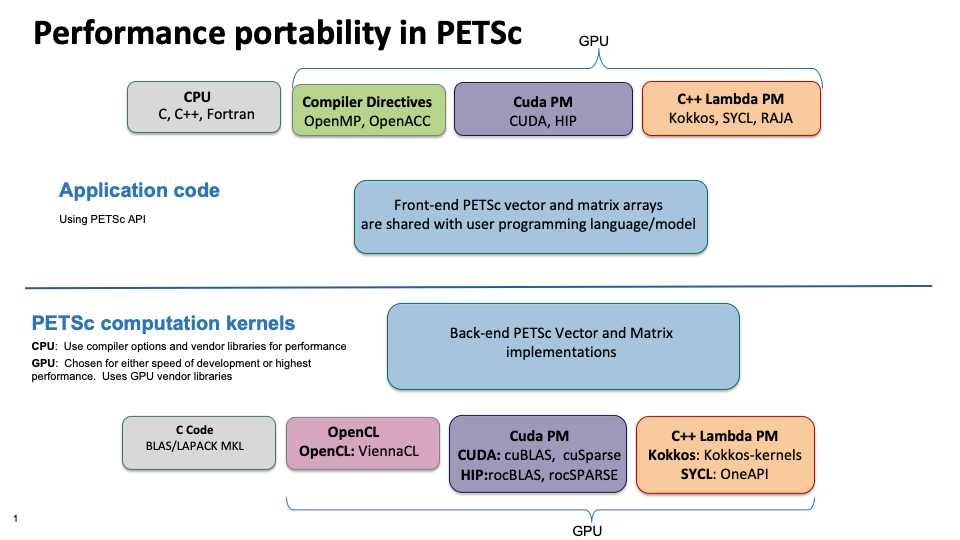
\includegraphics[trim = 0in .2in 1.7in .2in, clip, width=0.9\textwidth]{projects/2.3.3-MathLibs/2.3.3.06-PETSc-TAO/petsc_arch}
\caption{The PETSc/TAO architecture enables users to utilize a variety of programming
models for GPUs independently of PETSc's internal programming model.}
\label{fig:petsc-tao-fig}
\end{figure}

\begin{figure}
\centering
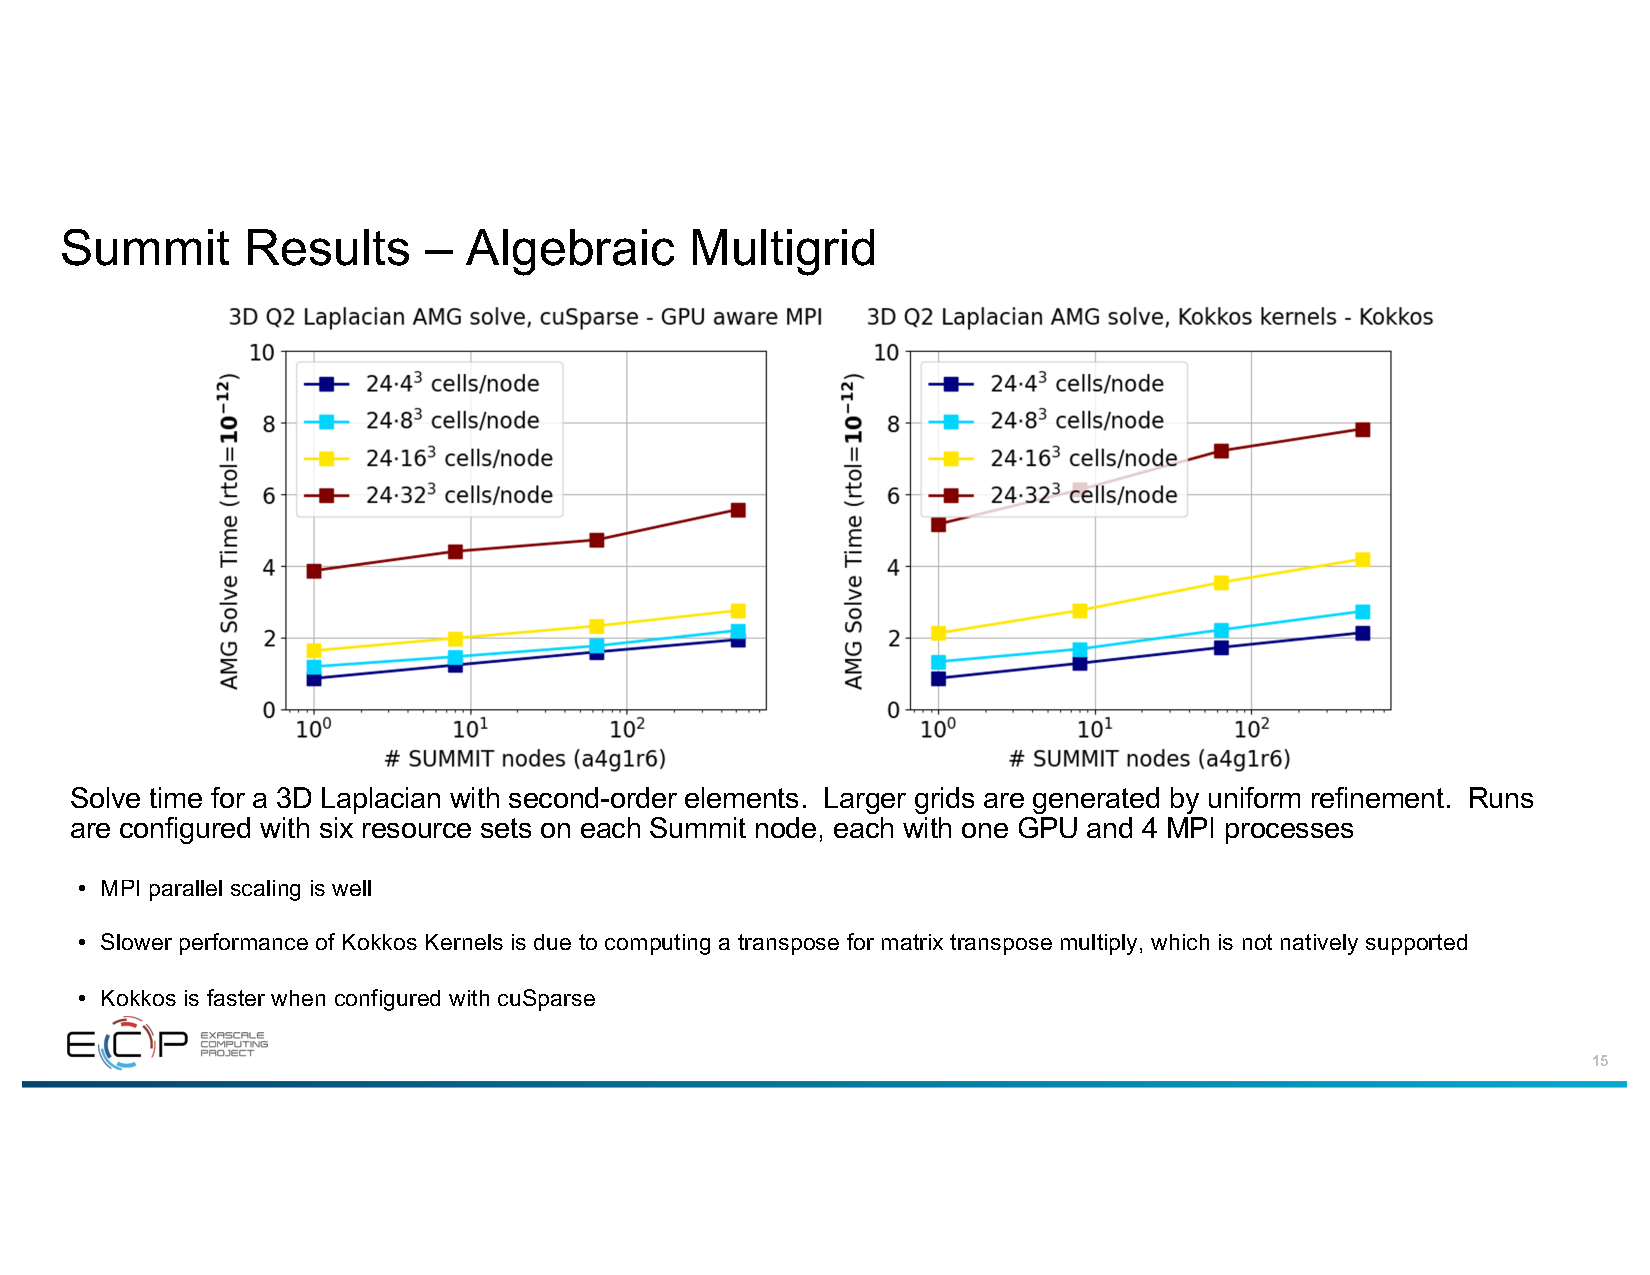
\includegraphics[trim = 1in 3.6in 1in 2in, clip, width=0.9\textwidth]{projects/2.3.3-MathLibs/2.3.3.06-PETSc-TAO/petsc_perf}
\caption{Solve time for a 3D Laplacian with second-order elements.  Larger grids are generated by uniform refinement.  Runs are configured with six resource sets on each Summit node, each with one GPU and 4 MPI processes.}
\label{fig:petsc-tao-perf}
\end{figure}

Our primary performance portability layer is based on Kokkos and KokkosKernels, which supports 
vector, matrix, and matrix-matrix operations.  We also have full support for a native CUDA 
backend and partial support for a native HIP and OpenCL backends.  Figure~\ref{fig:petsc-tao-perf}
demonstrates performance portability via a scaling study with PETSc/TAO’s built-in algebraic multigrid 
(AMG) solver, PCGAMG, using cuSPARSE and Kokkos (with KokkosKernels) back-ends on our most 
mature device, CUDA, where we obtain competitive performance.  The slower performance of 
KokkosKernels is due to computing a transpose for matrix transpose multiply, which is 
not yet natively supported in KokkosKernels.

The PETSc/TAO library has been compiled for Spock and Crusher and preliminary results have
been obtained using the accelerators and performance optimizations are being made.

The libEnsemble tools are based on python and makes calls to user-defined functions.  
The user-defined functions can use the accelerators on the compute nodes during their
evaluation.

\paragraph{Recent Progress}

In the past year, we have released PETSc/TAO 3.16 (available at \url{http://www.mcs.anl.gov/petsc}), which 
features enhanced GPU support.  We have full support for a Kokkos plus KokkosKernels backend for 
performance portability that includes vector, matrix, and matrix-matrix operations and full 
support for a native CUDA backend.  We have partial support for a native HIP and OpenCL 
backends.  We have been updating and profiling the GAMG solver, the native algebraic 
multigrid solver in PETSc, to use the enhanced GPU support.  Numerical results on
this work is available in \cite{mills2021toward}.  We have also been updating
our scalable communication layers, PetscSF, which allows us to use GPU-aware
MPI, thus allowing direct communication of data between Summit GPUs, bypassing 
the previously needed step of first copying the data to the CPU memory.  Numerical
results on this work is available in \cite{zhang2021petscsf}.

We have also released libEnsemble 0.7.2 (available at \url{https://github.com/Libensemble/libensemble}).
This release includes new generator functions and examples, improved testing across available platforms,
and a new tutorial.  A paper documenting libEnsemble and providing use cases is available
in \cite{hudson2021libensemble}.

\paragraph{Next Steps}

Our next efforts are:
\begin{enumerate}
  \item \textbf{Application readiness}: 
  We will complete a status review of our applications for the early access hardware.  We will 
  complete software quality initiatives related to the build system, architecture specific spack 
  recipes, and spack smoke tests for build and accelerator usage validation.
  \item \textbf{PETSc/TAO + Kokkos + KokkosKernels release}:
  We will release a version of PETSc/TAO with full Kokkos and KokkosKernels integration.  We will 
  provide a tutorial on these features, characterize the performance, and suggest optimizations 
  and best practices.  
  We will also make improvements to the PETSc/TAO GAMG solver and provide updated performance results.
  \item \textbf{libEnsemble + Balsam2 release}:
  We will release a version of libEnsemble with full Balsam2 support and updated API.
  We will follow continuous integration best practices and continue testing on pre-exascale DOE systems.
  \item \textbf{PETSc/TAO + Optimized communication layer release}:
  We will release a version of PETSc/TAO with an optimized communication layer for the early access systems.  
  This version will include support for AMGx on NVIDEA GPUs and a batch LU factorization and solver.
  We will optimize some numerical methods (such as methods in DMNetwork and numerical optimization methods) 
  to use the communication layer and better utilize the accelerators.
  We will provide initial benchmark results for GAMG and AMGx.
\end{enumerate}

